\documentclass[10pt, conference]{IEEEtran}
\usepackage{mdframed,graphicx,booktabs,textcomp,multirow,pgfplots,cite,tikz}
\usepackage{graphicx, csquotes}

\definecolor{bblue}{HTML}{4F81BD}
\definecolor{rred}{HTML}{C0504D}

\pgfplotsset{
    integral segments/.code={\pgfmathsetmacro\integralsegments{#1}},
    integral segments=3,
    integral/.style args={#1:#2}{
        ybar interval,
        domain=#1+((#2-#1)/\integralsegments)/2:#2+((#2-#1)/\integralsegments)/2,
        samples=\integralsegments+1,
        x filter/.code=\pgfmathparse{\pgfmathresult-((#2-#1)/\integralsegments)/2}
    }
}


\ifCLASSINFOpdf
 
\else
\fi

\hyphenation{Bug Fix Verification An Analysis of Pull Request Acceptance on the Tree-Structured Level}

\begin{document}
%
% paper title
% can use linebreaks \\ within to get better formatting as desired
\title{Bug Fix Verification: An Analysis of Pull Request Acceptance on the Tree-Structured Level}


% author names and affiliations
% use a multiple column layout for up to two different
% affiliations

\author{\IEEEauthorblockN{Yu-Ann Chen}
\IEEEauthorblockA{Institute of Software Research-Carnegie Mellon University\\Simmons College\\yuann.chen@simmons.edu}
}
\maketitle


\begin{abstract}
As society becomes more dependent on Open Source Software (OSS), it becomes more important to understand how we fix bugs. Pull requests serves as patch proposals to OSS and are accepted if it contributes to the project. But is there a way to understand the process of change and pull request acceptance in software? To tackle this problem, We wanted to understand what kind of structural data behavior is present in accepted pull requests, and ultimately, how this behavior can be used to classify and predict pull request acceptance. We collected pull request information from Github\textquotesingle s existing pull request system and processed file changes through our analysis. In the recent work around bug identification, we used what is known as naturalness and Change Distiller to mine more information about change in these files. As a result, two primary models were built, one using basic pull request information and the other using data mined from naturalness and Change Distiller. The advanced model reached an overall 70\% accuracy rate at predicting pull request acceptance, which exceeds the basic model\textquotesingle s accuracy rate. This approach has proven that structural analysis can be used to understand behavior of pull request acceptance. Ultimately, this work can be used to further understand what kind of bugs can be fixed automatically in OSS and how we can predict the evolution of OSS contribution.
\end{abstract}
\IEEEpeerreviewmaketitle

\section{Introduction}
\label{introduction}
The collaborative coding environment which OSS provides has lowered the barrier of entry for contributors~\cite{Yu}. Git, a version control system for software projects, has enabled developers to fork projects and update them locally. This allows developers to submit their local commits to the main branch of the repository. This is called a pull request. The process for patch submission has made social computing into a more formalized system. As contributors are able to track multiple changes throughout a distributed project, this collaborative environment has made it easier to integrate track issues and patches submissions for bug fixes.
\newline
\newline \indent It is obvious that bugs pose a huge problem in the modern practice of software development ~\cite{Asundi:2005:NEE:1082983.1083260}. As OSS becomes more prevalent in society, we are faced to trust thousands of developers around the world to build software. More importantly, the effects of bugs in OSS can impact thousands of users~\cite{Giachino:2014:CRD:2731750.2731754} and increase the social cost of software~\cite{Tassey.2002}. Therefore, bug management plays a major role in the design of the software itself and in its evolution. In OSS, pull requests act as patch proposals and are submitted to the core developers of the repository. However, 20-25\% of pull requests are reverted~\cite{Tsay:2014:LTE:2635868.2635882}.

We must understand what evidence can be provided to deduct a pull request acceptance. Recent studies have demonstrated techniques to understand changes in source code. Ray et al.~\cite{Ray:2016:NBC:2884781.2884848} shows that buggy code can be identified by measuring the source code\textquotesingle s naturalness. Naturalness refers to the repetitiveness and predictability of source code. Furthermore, Gall et al.~\cite{Gall:2009:CAE:1495795.1495953} created a technique that extracts fine-grained changes from the tree-structured level of code~\cite{1631103}. We hope to apply these techniques of understanding changes to assessing pull requests in OSS.

We use the information mined by naturalness and Change Distiller to find a correlation in pull request acceptance. We hypothesize that we can build a model that predicts whether a pull request would be accepted or rejected based on the changes made. We speculate that doing so will contribute further findings about the process of fixing bugs in OSS.

We evaluate the approach by computing prediction accuracy and cost effectiveness. This results will help us gain insights into the importance of the information provided on OSS service sites about pull requests. We also evaluate the performance metrics used in the approach by comparing its influence over the model\textquotesingle s prediction accuracy. 

We want to answer the following research questions:
\begin{mdframed} 
\begin{itemize}
\item \textbf{RQ1.} What structural data behavior is present in accepted pull requests?
\item \textbf{RQ2.} How can this behavior be used to classify and predict pull request acceptance?
\item \textbf{RQ3.} What is the most useful metric for predicting pull request acceptance?
\end{itemize}
\end{mdframed}

The rest of this paper is organized as follows: 
Section ~\ref{background} provides details on the techniques we are using in our prediction model. Section~\ref{approach} and ~\ref{evaluation} describes our approach towards collecting, extracting, and evaluating our data. In Section~\ref{discussion}, we present the results of our findings and address the research questions from Section~\ref{introduction}. We draw our conclusions in Section~\ref{conclusion} and discuss threats to validity and the future work of this paper.

\begin{figure*}
  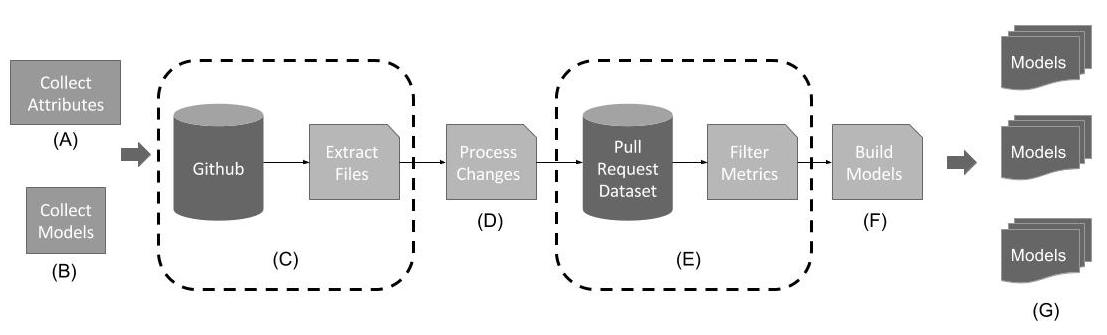
\includegraphics[width=\linewidth]{FlowChart.jpg}
  \caption{Overview of our approach. The letter of each step compliments the subsections of Section~\ref{approach}}
  \label{fig:FlowChart}
\end{figure*}

\section{Background}
\label{background}
We focus on understanding the process of pull requests as well as source code changes in this section. The following describes Github's process of submitting pull requests, the capabilities of naturalness and change distiller, and the reason for analyzing the data structured behavior of code.

\subsection{Github}
Github is a web-based version of git for developers to store repositories. Developers are able to use its pull request feature to submit bugs and patches. This web service ranks its most mature repositories by the amount of forks and stars given by other developers. While Github provides a webpage for displaying each repository and pull request submission, its large database is accessible through its Application Programming Interface (API). 

\subsection{Pull Request}
A pull request is a form of patch proposal to a OSS repository. When a developer forks a repository, he/she eventually will merge his/her changes to the master branch. The developer submits the commits with the patch(es) to the repository\textquotesingle s owner along with a commit message. The owner can then see the files changed in the repository as well as the specific source code lines changed. The owner can then merge the pull request, which implies that the pull request fixed a bug. The owner can also close the request which can indicate that the pull request was unable to fix a bug.

\subsection{Data Structured Behavior}
Existing source code changes are only analyzed at the line-level on Github. Data structured behavior is mined from analyzing source code at the Abstract Syntax Tree (AST) level. This means breaking up a source code into a tree and classifying the data into information which can be put into our predictive model. This allows for greater amounts of information that can be interpreted in many ways. For example, analyzing code at the data structured level has been used to understand coding conventions~\cite{Allamanis:2014:LNC:2635868.2635883}, code idioms, and coding style.

\subsection{Naturalness}
In Ray et al.~\cite{Ray:2016:NBC:2884781.2884848}, the naturalness of a file could be used to identify buggy code. Naturalness is measured by a code\textquotesingle s entropy and cross-entropy. This is done by using a language n-gram model which tracks the repetitiveness of tokens in source code. Entropy, the measure of repetitiveness and predictability is the output of analyzing source code. Cross-entropy is the measure of entropy over the code\textquotesingle s size (tokens). Ray et al. implicates that unnatural code is more likely to identify a big-fix commit.  Code with bug fixes are also more natural when repaired.

\subsection{Change-Distiller}
Gall et al.~\cite{Gall:2009:CAE:1495795.1495953} describe Change Distiller as a tree-differencing algorithm that mines fine-grained changes in source code at the tree-structured level. By taking two versions of a Java file, Change Distiller converts source code into Abstract Syntax Trees (AST). Using a tree-differencing algorithm, the difference between the two ASTs can be extracted and classified into data types and significant levels (the relevance of the change to the file). 

\section{Approach}
\label{approach}
This section, we will be discussing the methodology of answering our research questions. We first look at the models that could be built. Then, we look at the attributes that can be collected as performance metrics. Then, we collect pull request information from Github. We then run create multiple models for our evaluation.

\subsection{Collecting Attributes}
We form a list of promising attributes that indicate pull request acceptance. Each attribute was reasoned with potential in section~\cite{background}. There are a total of 176 attributes found in Github, Naturalness, and Change Distiller. Attributes that exist on pull request web pages, such as Github\textquotesingle s pull request feature are labeled as \enquote{Basic} under Type. Attributes found in Change Distiller and Naturalness are labeled as \enquote{Advanced} because these information are not available on pull request submission. These attributes are depicted in figure ~\cite{figureListOfMetrics} by attribute groups.

\begin{table*}[t]
  \centering
  \caption{List of Attributes (Metrics of Change)}
  \label{figureListOfMetrics}
  \begin{tabular}{l|rllllr}
    \toprule
    \textbf{Attribute Groups} & \textbf{\# of Attributes} & \textbf{Type}& \textbf{Origin} & \textbf{Level} & \textbf{Format} & \textbf{Range}\\ %colum names
    \midrule
    Number of Files & 1 & Basic & Github & Pull Request & Sum & 5,731 \\ %added row
    Lines of Code & 4 & Basic & Github & File & Sum, Average & 24,882 \\ %added row
    Files Changed & 4 & Basic & Github & Pull Request & Sum & 300 \\ %added row
    Naturalness & 8 & Advanced & Naturalness & File & Sum, Average & 1.01\\ %added row
    Significant Levels & 6 & Advanced & Change Distiller & File & Sum, Average &130,680 \\ %added row
     Structural Changes & 148 & Advanced & Change Distiller & File & Sum, Average & 7,798 \\ %added row
    \bottomrule
  \end{tabular}
  \break
  \newline
\textbf{Table \ref{figureListOfMetrics}:} This figure shows the attributes that are extracted from pull requests and their files. The origin describes where each attribute is derived from. The level depicts where the attribute is measured. The format describes how the attribute is interpreted for each pull request.
\end{table*}

\subsection{Collecting Machine Learning Algorithms}
We collect different types of algorithms: Random Forest, Logistic Model Tree (LMT), PART, Naive Bayes, and ZeroR. These classifiers were chosen because of the variety in handling the dataset of attributes. Random Forest serves to run efficiently on large data bases and has been known to handle thousands of input variables without variable deletion. LMT combines both a logistic regression and decision tree. PART is a algorithm that builds a partial C4.5 decision tree, which is used for continuing attribute value ranges, unavailable values, and entropy. Naive Bayes assumes attributes are independent. ZeroR serves as a baseline for other algorithms as it only predicts based on targets and not attributes.

\subsection{Extract File Changes in Dataset}
We request and collect the source code from each file\textquotesingle s rawURL using Github\textquotesingle s API. If a pull request was closed and merged, it would be classified as accepted. If a pull was closed and not merged, it would be classified as rejected. Our research questions only pertain to the technical and structure information of pull requests, which means we are not examining or collecting information about the developers or the pull request\textquotesingle s comments. The pull requests we collect are only Java files, due to the nature of Change Distiller. Therefore, the dataset collected were also filtered to not include pull requests containing non-java files.

\subsection{Process Changes}
We are using a language model called CodeMining-TreeLM to generate entropy level. Because all pull requests are from thirteen different repositories, we train 13 models with each repositories\textquotesingle s source code at an iteration of 400 times. Pull request\textquotesingle s files are matched with their respective project name, and using the serialized training set that was created by CodeMining-TreeLM, each file receives an entropy and cross-entropy value.

To process files through Change Distiller, each file is given to Change Distiller in two parts: the version before and after the pull request. Change Distiller then extracts changes and gives a sum of each change type from the file. 

The data mined with Naturalness and Change Distiller are saved in a text file that is specific to each pull requests. For example, a text file for Pull-Request-A may have information for 50 files because the pull request committed 50 files. The number of changes per file will be taken into account in the next step.

\subsection{Filtering Performance Metrics}
We create a script that parses through the text files of each pull request. The script selects the attributes we want as performance metrics, and the script formats the dataset into a file which will be the input for building a model. To answer our research questions, we adjust the attributes used from each database. This is why filtering the performance metrics is important to this approach.

\subsection{Building Models}
We use Weka, a model building application to process each file in a 10-fold cross validation. This classification process partitions the original dataset into ten subsamples. Nine subsamples are used for training and one subsample will be used for testing. Ultimately, the 10-fold cross validation reduces the sensitivity of the model\textquotesingle s performance to new data. By having Weka distribute the data for both the training set and the testing of the model, we will not receive surprising results when it makes new predictions for data it has never seen.

\subsection{Data-Analysis}
Using the model built by Weka, We create a confusion matrix to calculate precision, recall, and the area under the curve (AUC). This analysis is then used to calculate the model\textquotesingle s prediction accuracy.

\section{Evaluation}
\label{evaluation}
In this section, we will be reviewing the evaluations of the approach we took. This constitutes the validity of the dataset, the performance of our predictive models, and the usefulness of each attribute.

\subsection{Validity of Data}
The pull requests collected are validated based on the repository\textquotesingle s maturity. We collect these pull requests from the top 13 Java projects with the most forks, stars, and pull requests. We successfully collect 2,247 pull requests with a balanced ratio of accepted to rejected pull requests of 55 to 45.

\subsection{Predictability Accuracy Comparison}
We apply our approach to the dataset we have collected and built two models: The basic model and advanced model. The basic model encompasses only the attributes from Github, and the advanced model has a combination of the basic model\textquotesingle s attributes, naturalness, and structural changes. The coin toss model is built based on the the number of accepted and rejected pull requests over a random 50/50\% probability in predictability. The advanced model is compare to the coin toss model to validate the balance of accepted and rejected pull requests in the dataset. Since the basic model uses data from only Github, it will serve as a baseline for evaluating how the advanced model compares to existing methods of predicting pull request acceptance.

\subsection{Validity of Machine Learning Classifiers}
To validate the classifying models used, We took five different types of classifier and measured its performance over the AUC. We took the same data from the advanced model and implemented different algorithms along with Random Forest: LMT, PART, Naive Bayes, and ZeroR. We then compare both the accuracy and the ROC Area. We will test the five classifiers on three of the following datasets: Basic, Advanced, and Basic + Advanced.

\section{Discussion of Results}
\label{discussion}
\subsection{Research Questions \#1}
Table~\cite{figureListOfMetrics} provides a list of attributes that are found in pull requests. Because pull request vary in the number of files, each pull requests differ in the sum of attributes (i.e. lines of code, naturalness, etc.). Therefore, we use both the sum and average over the number of files for attributes that depend on the number of files. This is indicated in the format column of Table~\cite{figureListOfMetrics}.

Structural Changes have the most number of attributes. This is because of the classification of data structure found in Java in Change Distiller. However, the significant levels have the largest range of all attribute groups. This makes sense because each change in line of code for each file is given a low, medium, or high significant levels. Naturalness has the lowest range because naturalness is measured with the difference in $10^{-10}$.

Structural changes have the most number of attributes of the group of attributes. Unlike lines of code changes, structural changes presents more ways to interpret changes. The variety of data helps with creating a model that accurately predicts pull requests.

Although we want to learn whether these attributes are correlated with pull request acceptance, this research question serves to find existing attributes of each pull request. We analyze the "usefulness" of these attributes in Research Question \#3.

\begin{table}[h!]
  \centering
  \caption{Accuracy of Predictive Models}
  \label{figurePredictionModels}
  \begin{tabular}{lrrr}
    \toprule
    \textbf {Model} & \textbf{Accuracy} & \textbf{Precision} & \textbf{Recall}\\ %colum names
    \midrule
    Coin Toss & 48\% & - & - \\ %added row
    Basic & 58\% & 0.58 & 0.77\\ %added row
    Advanced & 70\% & 0.72 & 0.91\\ %added row
    Basic + Advanced & 69\% & 0.64 & 0.68\\ %added row
    \bottomrule
  \end{tabular}
  \break
  \break
\textbf{Table \ref{figurePredictionModels}:} Each model was measured by how accurate it was able to correctly classify pull requests. Precision and recall are also used to evaluate the performance of each model.
\end{table}

\begin{table}[h!]
  \centering
  \caption{Performance of Classifiers}
  \label{figureClassifers}
  \begin{tabular}{c|lrr}
    \hline
    \textbf {Dataset} & \textbf{Classifer} & \textbf{Accuracy} & \textbf{ROC Area}\\
    \hline
    \multirow{5}{*}{Basic [13]}
    				& \multicolumn{1}{l}{Random Forest} & \multicolumn{1}{r}{58\%} & \multicolumn{1}{r}{0.61} \\\cline{2-4}
                                 & \multicolumn{1}{l}{LMT} & \multicolumn{1}{r}{59\%} & \multicolumn{1}{r}{0.59} \\\cline{2-4}
                                 & \multicolumn{1}{l}{PART} & \multicolumn{1}{r}{58\%} & \multicolumn{1}{r}{0.61} \\\cline{2-4}
                                 & \multicolumn{1}{l}{Naive Bayes} & \multicolumn{1}{r}{58\%} & \multicolumn{1}{r}{0.56} \\\cline{2-4}
                                 & \multicolumn{1}{l}{ZeroR} & \multicolumn{1}{r}{54\%} & \multicolumn{1}{r}{0.50} \\\hline
    \multirow{5}{*}{Advanced [163]} 
    				& \multicolumn{1}{l}{Random Forest} & \multicolumn{1}{r}{61\%} & \multicolumn{1}{r}{0.65} \\\cline{2-4}
                                 & \multicolumn{1}{l}{LMT} & \multicolumn{1}{r}{59\%} & \multicolumn{1}{r}{0.59} \\\cline{2-4}
                                 & \multicolumn{1}{l}{PART} & \multicolumn{1}{r}{59\%} & \multicolumn{1}{r}{0.60} \\\cline{2-4}
                                 & \multicolumn{1}{l}{Naive Bayes} & \multicolumn{1}{r}{51\%} & \multicolumn{1}{r}{0.49} \\\cline{2-4}
                                 & \multicolumn{1}{l}{ZeroR} & \multicolumn{1}{r}{54\%} & \multicolumn{1}{r}{0.50} \\\hline
    \multirow{5}{*}{Basic + Advanced [176]} 
    				& \multicolumn{1}{l}{Random Forest} & \multicolumn{1}{r}{61\%} & \multicolumn{1}{r}{0.65} \\\cline{2-4}
                                 & \multicolumn{1}{l}{LMT} & \multicolumn{1}{r}{60\%} & \multicolumn{1}{r}{0.58} \\\cline{2-4}
                                 & \multicolumn{1}{l}{PART} & \multicolumn{1}{r}{57\%} & \multicolumn{1}{r}{0.60} \\\cline{2-4}
                                 & \multicolumn{1}{l}{Naive Bayes} & \multicolumn{1}{r}{55\%} & \multicolumn{1}{r}{0.54} \\\cline{2-4}
                                 & \multicolumn{1}{l}{ZeroR} & \multicolumn{1}{r}{54\%} & \multicolumn{1}{r}{0.50} \\\hline
  \end{tabular}
  \break
  \break
\textbf{Table III:} Each model was measured by how accurate it was able to correctly classify pull requests. Precision and recall are also used to evaluate the performance of each model.
\end{table}

\subsection{Research Question \#2}
We show that fine-grained source code changes in pull request can lead to improved models for predicting pull request acceptance. In Table II, the basic model received an accuracy rate of 58\% and the advanced model generated a 69\% accuracy rate. With the addition of the behavior presented in Research Question 1, the model was able to predict at a 11\% higher accuracy. We further evaluated the performance of the models by comparing their precision and recall.

The advanced model had a 0.14 higher precision and recall. Based on these results, we can answer the question: The structured behavior of accepted pull requests can predict pull request acceptance by creating a model using the Random Forest algorithm.

The predictive model with the advanced dataset exceeded all other models in accuracy. The coin toss also validates the balance of the dataset. We are able to compare the predictive model with the advanced dataset to both the coin toss and the basic dataset, which represents the existing information that\textquotesingle s available for developers to use when responding to pull requests.

In understanding the performance of classifiers, we use the ROC Area as an indicator of cost-effectiveness of each algorithm. Random Forest performed the greatest, which is indicated by the ROC Area. ZeroR performed in the worst with a 0.50 ROC Area. This is expected because ZeroR uses a statistical "coin-toss" to determine its predictions. Random Forest has been known to work well with datasets that are not fully correlated with each other. LMT also performed as well as Random Forest. Although LMT suffers from not implementing randomness into its algorithm. 

Table~\ref{figureClassifers} shows a ranking of classifiers for each dataset. In all dataset, Random Forest performed the best in both accuracy and ROC Area. For the Advanced and Basic + Advanced dataset, Random Forest predicted at a 61\% accuracy. ZeroR had the lowest accuracy of 54\% in all three datasets. This is predicted because ZeroR depicts a coin-toss behavior. However, it still exceeds the coin toss accuracy. LMT, PART, and Naive Bayes 

\begin{table}[h!]
  \centering
  \caption{Usefulness of Metrics}
  \label{figureUsefulness}
  \begin{tabular}{p{0.5cm} l | l r r}
    \toprule
    \textbf{Rank}&\textbf {Metric} & \textbf{Type} & \textbf{Accuracy} & \textbf{Difference}\\ %colum names
    \midrule
    1 & Avg. FOR\_INCR & Advanced & 54.34\% & -15.66\%\\ %added row
    2 &  Avg. TYPE\_PARAMETER & Advanced & 54.52\% & -15.48\%\\ %added row
    3 & Avg. WILDCARD\_TYPE & Advanced & 54.56\% & -15.44\%\\  %added row
     174 & Files Modified & Basic & 61.59\% & -8.41\%\\ %added row
     175 & Number of Files & Basic & 61.59\% & -8.41\%\\%added row
     176 & Files Added & Basic & 61.64\% & -8.46\%\\  %added row
    \bottomrule
  \end{tabular}
  \break
  \break
\textbf{Table ~\ref{figureUsefulness}:} Each metric used in this paper is presented with an accuracy of a predictive model without the metric. The difference of each metric shows the increase/decrease in accuracy when it is missing from the advanced model. This table shows the influence of each metric over the predictive model.
\end{table}

\subsection{Research Question \# 3}
In our approach, we created various models with the same data but with a unique metric missing. Taking the accuracy of each model, we are able to measure the influence which each metric has on the overall advance model\textquotesingle s accuracy. I Beyond the metrics found in the basic model, our findings also showed that the entropy metrics and structural changes had the biggest influence over the accuracy rate. The model which excluded entropy metrics had the biggest decrease in accuracy rate of 4\%. We pose that the \enquote{usefulness} of a metric is defined by its positive influence over the overall accuracy. We can now answer the third research question: Entropy and structural changes had the most influence over the accuracy of the advanced model. 

In Table ~\ref{figureUsefulness}, the three most useful metrics are structural changes found in the advanced dataset. These metrics are also average calculations of specific structural change frequencies. All three metrics had a significant difference on the accuracy on 15.44\% to 15.66\%, which means the accuracy rate was decreased to 54.34\% - 54.56\% with the absence of these metrics. We can conclude that average calculations  of structural changes are the most useful. The metrics that had the least influence on the predictive model were found in from the basic dataset. This means that they had little influences over the predictive model.

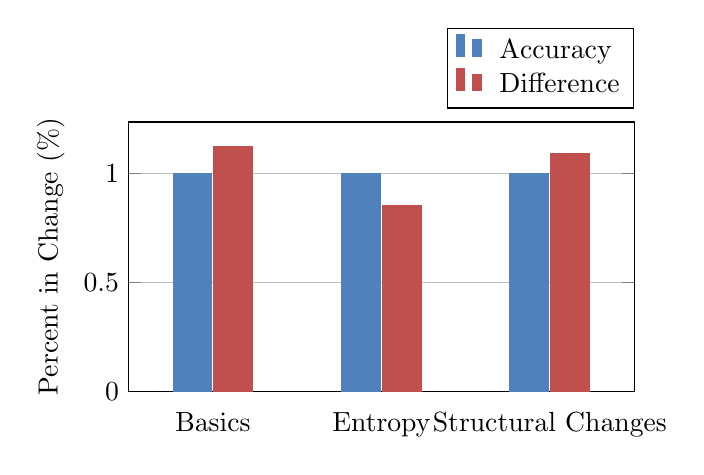
\begin{tikzpicture}
    \begin{axis}[
        width  = 8cm,%*\textwidth,
        height = 5cm,
        major x tick style = transparent,
        ybar=2*\pgflinewidth,
        bar width=14pt,
        ymajorgrids = true,
        ylabel = {Percent in Change (\%)},
        symbolic x coords={Basics,Entropy,Structural Changes},
        xtick = data,
        scaled y ticks = false,
        enlarge x limits=0.25,
        ymin=0,
        legend cell align=left,
        legend style={
                at={(1,1.05)},
                anchor=south east,
                column sep=1ex
        }
    ]
        \addplot[style={bblue,fill=bblue,mark=none}]
            coordinates {(Basics, 1.0) (Entropy,1.0) (Structural Changes,1.0)};

        \addplot[style={rred,fill=rred,mark=none}]
             coordinates {(Basics,1.123) (Entropy,0.85) (Structural Changes,1.09)};

        \legend{Accuracy,Difference}
    \end{axis}
    \end{tikzpicture}
\newline \small \textbf{Table II:} The accuracy bars compare the accuracy rate of each model missing the group of metrics (see Figure VII for a table version of this figure). The metric grouping with the  least accurate model in this graph should be interpreted as the most useful metrics group. The difference bar shows the increase and decrease of the prediction accuracy compared to the advanced model. Metric groups with positive difference bars had negative influences over the model (this is vice versa for negative difference bars).


\section{Conclusion}
\label{conclusion}
Throughout this paper, we analyzed what change occurs in pull requests. The following are the results we have concluded:

\begin{mdframed} 
\begin{itemize}
\item \textbf{RQ1.} High entropy and structural changes are present in accepted pull requests.
\item \textbf{RQ2.} The model with the these behavior as performance metrics performed better with a higher accuracy rate.
\item \textbf{RQ3.} Entropy and structural changes are also the biggest influence in the model.
\end{itemize}
\end{mdframed}

Overall, the nature of this project contributes findings to understanding the nature of social computing, specifically OSS. 

\subsection{Threats to Validity}
This project faces one particular threat to its validity. In the nature of bug fixing and the definition of a bug, a pull request acceptance may not indicate whether a pull request fixed a bug. This could alter the collected data and detour from the high-level purpose of the project. However, since the advanced model proved to have a high predicting accuracy, this threat may not as be detrimental as we thought. Additional threat to  our data\textquotesingle s validity includes our limiting dataset. It is evident that Java projects are more explicit with its data structure than other programming languages. In terms of practicality, the approach we took with Java projects may not work for the OSS written in other languages.

\subsection{Future Work}
We hope to expand this work to more programming languages. This would involve understanding Change Distiller\textquotesingle s algorithm and implementing its AST converter to languages like C and Python. We will continue to pursue our high-level goal of understanding the process of bug fixing in OSS. *We will add more future work here*

We hope that our approach ~\cite{Giachino:2014:CRD:2731750.2731754} is not limited to Change Distiller and Naturalness. Our predictive model can be enhanced by analyzing the repository\textquotesingle s pull request history for patterns in acceptable structural changes [reference]. If we are able to take this approach, our predictive model may be able to classify future changes and ultimately future bugs. ~\cite{Yu}

\section*{Acknowledgment}
This project was funded by the National Science Foundation. We thank Claire De Goues for her insightful suggestions and advisory.

\bibliography{myBib}
\bibliographystyle{plain}


% that\textquotesingle s all folks
\end{document}

